\documentclass[dvipdfmx,11pt]{beamer}

%\usepackage{bxdpx-beamer}
\usepackage{listings,jlisting}
\usepackage{graphicx,xcolor} %文字の色
\usepackage[deluxe]{otf}
\usepackage{txfonts}


\usetheme{Warsaw}

\newcommand{\code}[1]{\lstinline[basicstyle=\ttfamily]{#1}}
\renewcommand{\kanjifamilydefault}{\gtdefault}
\renewcommand{\bibname}{参考文献}
\setbeamersize{text margin left=1.5em,text margin right=1.5em} %文字間の余白調整
\setbeamertemplate{navigation symbols}{} %アイコン消去
\setbeamertemplate{footline}[frame number] %フレーム番号表示
\useoutertheme{shadow}
\usefonttheme{professionalfonts} %数式文字のLaTeX化


\title{解集合プログラミングを用いたグラフ彩色問題の解法に関する考察}
\author{101830314 春田 穂高}
\institute{番原研究室}
\date{2021年度 卒業研究発表会\\2022年2月18日}

\begin{document}
%%%%%%%%%%%%%%%%%%%%%%%%%%%%%%%%%%%%%%%%%%%%%%%%%%%%%%%%%%%%%%%%%%%
\frame{\maketitle}
%%%%%%%%%%%%%%%%%%%%%%%%%%%%%%%%%%%%%%%%%%%%%%%%%%%%%%%%%%%%%%%%%%%
\begin{frame}{グラフ彩色問題と関連問題}
 \begin{itemize}
  \item \alert{グラフ彩色問題}
        \begin{itemize}
	 \item 与えられた有限無向グラフ$G$の隣接する頂点が
	       同色にならないように各頂点を塗りわけるときに,
	       必要となる最小の色数を求める問題.
	 \item 最適化コンパイラのレジスタ割り付けや
	       無線の周波数割り当て等の応用がある.
        \end{itemize}
  \item \alert{グラフ彩色判定問題}
        \begin{itemize}
         \item 自然数$k\geq 3$について,
	       グラフ$G$が$k$色以下で彩色可能かどうかを決定する問題.
        \end{itemize}
 \end{itemize}

 \begin{alertblock}{}
  \centering
  グラフ彩色問題はNP困難,グラフ彩色判定問題はNP完全である.
 \end{alertblock}
\end{frame}

%%%%%%%%%%%%%%%%%%%%%%%%%%%%%%%%%%%%%%%%%%%%%%%%%%%%%%%%%%%%%%%%%%%
\begin{frame}{グラフ彩色問題と関連問題}
 \begin{itemize}
  \item \alert{グラフ彩色における同色頂点数最小化問題}
        \begin{itemize}
         \item グラフ彩色判定問題の実行可能解のうち,
	       同色(例えば,赤色)で塗られる頂点数の最小値を求める問題である.
        \end{itemize}
  \item \alert{グラフ彩色における同色頂点数最大化問題}
        \begin{itemize}
         \item グラフ彩色判定問題の実行可能解のうち,
	       同色(例えば,赤色)で塗られる頂点数の最大値を求める問題である.
        \end{itemize}
  \item \alert{グラフ彩色における多色頂点数最大化問題}
        \begin{itemize}
         \item グラフ彩色判定問題の制約を満たしつつ,
	       多色(2色以上)で塗られる頂点数の最大値を求める問題である.
         \item この問題の最適解は,基のグラフ彩色判定問題の複数の実行可能解に
               対応し,基の問題の圧縮解とみなすことができる.
        \end{itemize}
 \end{itemize}

 \begin{alertblock}{}
  \centering
  本研究では,グラフ彩色に関する最適化問題を対象とする.%%% あってますか?
 \end{alertblock}
\end{frame}

%%%%%%%%%%%%%%%%%%%%%%%%%%%%%%%%%%%%%%%%%%%%%%%%%%%%%%%%%%%%%%%%%%%
\begin{frame}{ \code{McGregor} グラフ[Knuth2015]}
 \begin{exampleblock}{5次の \code{McGregor} グラフ}
  \begin{center}
   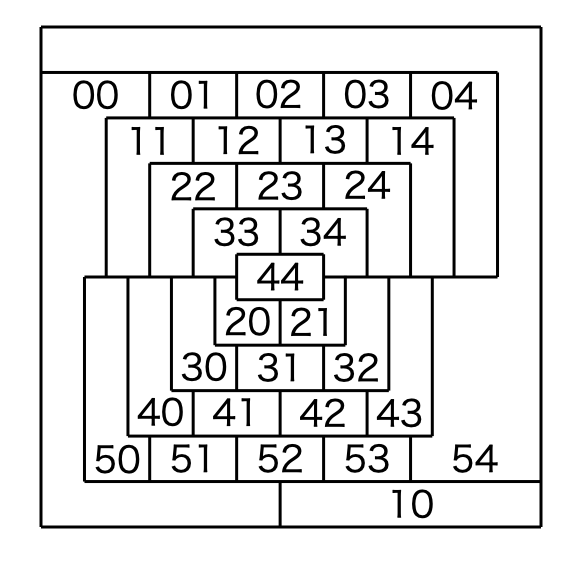
\includegraphics[scale=0.2]{fig/order5.png}
  \end{center}
 \end{exampleblock}

 \begin{itemize}
  % \item D.~E~.Knuthの教科書
  %        The Art of Computer Programming~\cite{Knuth:TAOCP:SAT}
  %        に記載されているグラフである.
  \item \code{McGregor} グラフの各区画が頂点に,区画の隣接関係が辺に対応.
  \item グラフを構成する頂点や辺は次数$n$によって定まり,
	頂点数は$N=n*(n+1)$個,辺数は$3N-6$本である.\cite{Knuth:TAOCP:SAT}
  \item 次数$n$に関わらず,4色で彩色可能であることが知られている.
 \end{itemize}
\end{frame}

%%%%%%%%%%%%%%%%%%%%%%%%%%%%%%%%%%%%%%%%%%%%%%%%%%%%%%%%%%%%%%%%%%%
\begin{frame}{多色頂点数最大化問題}
 \begin{tabular}{cc}
  \begin{minipage}[t]{0.5\linewidth}
   \centering
   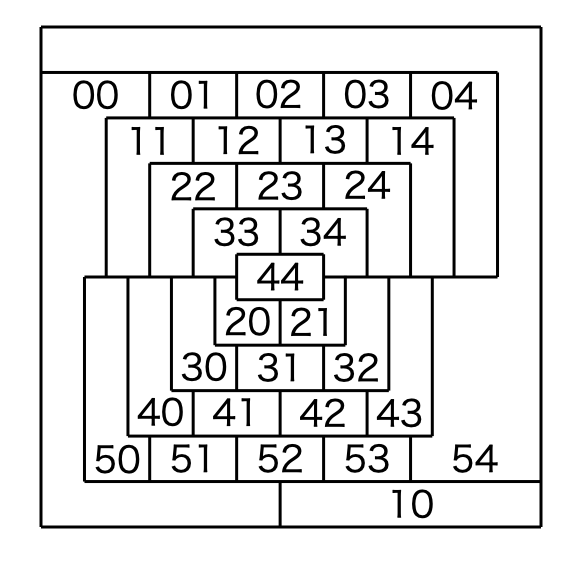
\includegraphics[scale=0.2]{fig/order5.png}
  \end{minipage}
  \begin{minipage}[t]{0.5\linewidth}
   \centering
   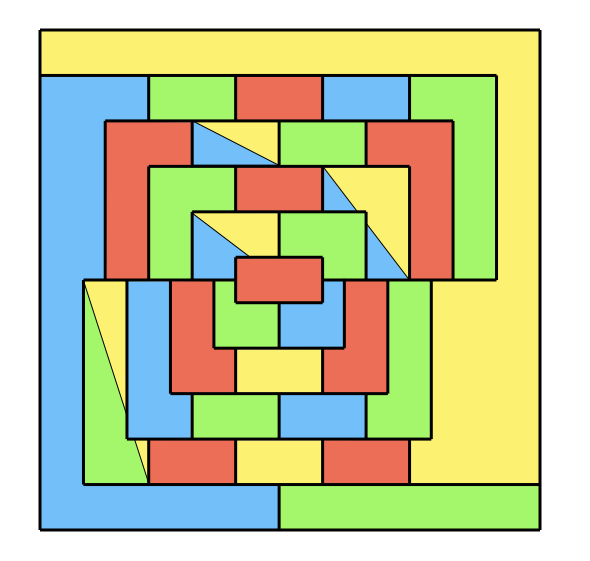
\includegraphics[scale=0.2]{fig/order5_mult.png}
  \end{minipage}
 \end{tabular}

 \begin{exampleblock}{}
  5次の McGregorグラフが与えられ,4色以下で塗り分けるときに,
  多色(2色以上)で塗られる頂点数の最大値を求める問題を考える.
 \end{exampleblock}

 \begin{itemize}
  \item 最適値は4で,
	頂点番号\code{12}, \code{24}, \code{33}, \code{50}
	が2色で彩色できる.
  \item この最適解は,色数4のグラフ彩色判定問題における
	\alert{16}個の実行可能解の圧縮解とみなすことができる.
 \end{itemize}
\end{frame}

%%%%%%%%%%%%%%%%%%%%%%%%%%%%%%%%%%%%%%%%%%%%%%%%%%%%%%%%%%%%%%%%%%%
\begin{frame}{解集合プログラミング(Answer Set Programming; ASP)}
 \begin{itemize}
  \item \alert{ASP}は,論理プログラミングから派生した
        比較的新しいプログラミングパラダイムである.
  \item \alert{ASP言語}は,一階論理に基づいた知識表現言語の一種である.
  \item \alert{ASPシステム}は,論理プログラムから
        安定モデル意味論~{\scriptsize[Gelfond and Lifschitz, '88]}
        に基づく解集合を計算するシステムである.
  \item 近年,SAT技術を利用する高速なASPシステムが開発され,
        様々な分野への実用的な応用が急速に拡大している.
 \end{itemize}
 
 \begin{alertblock}{グラフ彩色判定問題に対してASPを用いる利点}
  \begin{itemize}
   \item ASP言語の高い表現力により,記号制約を簡潔に記述可能.
   \item 充足不能コアを用いた最適化探索が可能.
   \item 高速ASPシステムを用いた高速な解探索,解列挙が可能.
  \end{itemize}
 \end{alertblock}
\end{frame}

%%%%%%%%%%%%%%%%%%%%%%%%%%%%%%%%%%%%%%%%%%%%%%%%%%%%%%%%%%%%%%%%%%%
\begin{frame}{研究目的と内容}
 \begin{alertblock}{研究目的}%%% 自分で書き換えてみてほしい
  \begin{itemize}
   \item グラフ彩色判定問題とその関連問題に対して,
         ASP符号化を提案し,評価する.
   \item 得られた解を利用した,グラフ彩色問題の実行可能解の圧縮.
  \end{itemize}
 \end{alertblock}

 \begin{block}{研究内容}
  \begin{enumerate}
   \item \structure{グラフ彩色判定問題とその関連問題を解くASP符号化の考案}
         \begin{itemize}
          \item %color符号化,
                minimize符号化,
                maximize符号化,mult符号化.
         \end{itemize}
   \item \structure{ベンチマーク問題を用いた評価実験}
         \begin{itemize}
%          \item McGregorグラフを表すベンチマーク問題(計138問)を新たに作成.
          \item グラフ彩色判定問題,同色頂点数最小化問題,
                同色頂点数最大化問題,多色頂点数最大化問題
                のそれぞれに対して実験を行った.
          \item グラフ彩色判定問題の実行可能解の全列挙を行った.(発表省略)
         \end{itemize}
   \item \structure{グラフ彩色判定問題の実行可能解の圧縮についての調査}
         \begin{itemize}
          \item 多色頂点数最大化問題の一つの最適解が表現する,
		基のグラフ彩色判定問題の実行可能解の数を調査した.
         \end{itemize}
  \end{enumerate}
 \end{block}
\end{frame}

%%%%%%%%%%%%%%%%%%%%%%%%%%%%%%%%%%%%%%%%%%%%%%%%%%%%%%%%%%%%%%%%%%%
\begin{frame}{考案するASP符号化}
 \begin{block}{グラフ彩色判定問題の表現}
  与えられた有限無向グラフ$G$と自然数$k\geq 3$について,
  以下2つの制約を満たすように$G$の各頂点を
  $k$色以下で彩色可能かを決定する問題.
  \begin{itemize}
   \item $G$の各頂点は一つの色で彩色される.(彩色制約)
   \item $G$の隣接する頂点は同色で彩色されない.(隣接制約)
  \end{itemize}
 \end{block}
 \begin{enumerate}
   \item \structure{color符号化}:
         \begin{itemize}
          \item グラフ彩色判定問題の彩色制約と隣接制約を簡潔に表現した.
         \end{itemize}
  \item \alert{minimize符号化}:%%% 同色頂点数最小化問題と記述したい
        \begin{itemize}
         \item color符号化をベースに,
               ASPの最小化関数~\texttt{\#minimize} を用いて,
	       同色で塗られる頂点数を最小化する目的関数を追加.
        \end{itemize}
  \item \alert{maximize符号化}:%%% 同色頂点数最大化問題と記述したい
        \begin{itemize}
         \item color符号化をベースに,
               ASPの最大化関数~\texttt{\#maximize} を用いて,
	       同色で塗られる頂点数を最大化する目的関数を追加.
        \end{itemize}
  \item \alert{mult符号化}:%%% 多色頂点数最大化問題と記述したい
        \begin{itemize}
         \item color符号化をベースに,
	       1つの頂点を多色で彩色できるように彩色制約の上限を緩和.
         \item ASPの最大化関数~\texttt{\#maximize} を用いて,
	       多色で彩色できる頂点数を最大化する目的関数を追加.
        \end{itemize}
 \end{enumerate}
\end{frame}

%%%%%%%%%%%%%%%%%%%%%%%%%%%%%%%%%%%%%%%%%%%%%%%%%%%%%%%%%%%%%%%%%%%
% \begin{frame}{実験概要}
%  \begin{block}{}
%   考案した符号化の有効性を評価するために各問題の実験を行った.
%  \end{block}

% \begin{itemize}
%  \item \structure{ベンチマーク問題}: order~3$\sim$140のMcGregorグラフ(計138問)
%  \item \structure{ASPシステム}: \textit{clingo}-5.5.0
%  \item \structure{実験環境}: Mac mini Intel Core i7 3.2GHz 64GBメモリ
%  \item \structure{制限時間}: 
%        \begin{itemize}%%% 問題に対してでなくて良いか
%         \item color符号化: 30分
%         \item minimize,maximize,mult符号化: 1時間
%        \end{itemize}
% \end{itemize}  

%  \begin{alertblock}{color符号化の実験結果}
%   order~3$\sim$138の計136問について4彩色可能であると判定できた.
%  \end{alertblock}
 
% \end{frame}

%%%%%%%%%%%%%%%%%%%%%%%%%%%%%%%%%%%%%%%%%%%%%%%%%%%%%%%%%%%%%%%%%%%
\begin{frame}{実験概要}
 \begin{block}{}
  考案した符号化の有効性を評価するために各問題の実験を行った.
 \end{block}

\begin{itemize}
 \item \structure{対象とする問題}:
       \begin{enumerate}
        \item グラフ彩色判定問題: $N$次の\code{McGregor}グラフ ($3 \leq N\leq 140$)
              \begin{itemize}
               \item \structure{制限時間}: 30分/問
              \end{itemize}
        \item 同色頂点数最小化問題: $N$次の\code{McGregor}グラフ ($3 \leq N\leq 20$)%%% BB法とUSC法は?
              \begin{itemize}
               \item \structure{制限時間}: 1時間/問
              \end{itemize}
        \item 同色頂点数最大化問題: $N$次の\code{McGregor}グラフ ($3 \leq N\leq 38$)%%% BB法とUSC法は?
              \begin{itemize}
               \item \structure{制限時間}: 1時間/問
              \end{itemize}
        \item 多色頂点数最大化問題: $N$次の\code{McGregor}グラフ ($3 \leq N\leq 15$)%%% BB法とUSC法は?
              \begin{itemize}
               \item \structure{制限時間}: 1時間/問
              \end{itemize}
       \end{enumerate}
 \item \structure{ASPシステム}: \textit{clingo}-5.5.0
 \item \structure{実験環境}: Mac mini Intel Core i7 3.2GHz 64GBメモリ
\end{itemize}  

 \begin{alertblock}{グラフ彩色判定問題の実験結果}
  $3 \leq N\leq 138$ の計136問は,
  制限時間内に実行可能解を求められた.
 \end{alertblock}
\end{frame}

%%%%%%%%%%%%%%%%%%%%%%%%%%%%%%%%%%%%%%%%%%%%%%%%%%%%%%%%%%%%%%%%%%%
\begin{frame}{同色頂点数最小化問題の実験結果(最適値と最良値)}
 \begin{block}{}
  \structure{問題}: $N$次の\code{McGregor}グラフ ($3 \leq N\leq 20$: 計18問)
 \end{block}

 \begin{center}
  \begin{tabular}{r|c|c}
 %n& f(n)\\
 N&BB &USC\\
 \hline
 3&2*&2*\\
 4&2*&2*\\
 5&3*&3*\\
 6&4*&4*\\
 7&5*&5*\\
 8&7*&7*\\
 9&7*&7*\\
 10&7*&7*\\
 11&8*&8*\\
 12&9*&9*\\
 13&10*&10*\\
 14&12&\textbf{12*}\\
 15&\textbf{12}&49\\
 16&16&\textbf{12*}\\
 17&21&\textbf{\textcolor{red}{13*}}\\
 18&19&\textbf{\textcolor{red}{14*}}\\
 19&\textbf{20}&58\\
 20&\textbf{22}&59\\\hline
\end{tabular}


 \end{center}

 \begin{itemize}
  \item BB法が優れていた問題は3問,
        USC法が優れていた問題は4問.
  \item BB法は11問,USC法は15問において,
	最適値を求ていた.
  \item $N = 17,18$ の2問について
	新たに最適値を発見することができた.
 \end{itemize}
\end{frame}

%%%%%%%%%%%%%%%%%%%%%%%%%%%%%%%%%%%%%%%%%%%%%%%%%%%%%%%%%%%%%%%%%%%
\begin{frame}{同色頂点数最大化問題の実験結果(最適値と最良値)}
 \begin{block}{}
  \structure{問題}: $N$次の\code{McGregor}グラフ ($3 \leq N\leq 38$: 計36問)
 \end{block}
 
 \begin{center}
  \begin{table}[t]\scriptsize
%\renewcommand{\arraystrech}{1.2}
\begin{tabular}{r|cc||r|cc||r|cc}
 \hline
 %n& g(n)\\
 N&BB &USC&N&BB&USC&N&BB&USC\\
 \hline
 3&4*&4*&    15&71&\textbf{77*}&
 27&\textbf{185}&180 \\
 4&6*&6*&    16&71&\textbf{88*}&
 28&199&\textbf{\textcolor{red}{266*}} \\
 5&10*&10*&    17&76&\textbf{\textcolor{red}{99*}}&
 29&221&\textbf{\textcolor{red}{285*}} \\
 6&13*&13*&    18&91&\textbf{\textcolor{red}{111*}}&
 30&224&\textbf{\textcolor{red}{305*}} \\
 7&17*&17*&    19&92&\textbf{\textcolor{red}{123*}}&
 31&247&\textbf{\textcolor{red}{325*}} \\
 8&23*&23*&    20&109&\textbf{\textcolor{red}{137*}}&
 32&255&255 \\
 9&28&\textbf{28*}&    21&121&\textbf{\textcolor{red}{150*}}&
 33&\textbf{280}&278 \\
 10&35&\textbf{35*}&    22&122&\textbf{\textcolor{red}{165*}}&
 34&296&\textbf{\textcolor{red}{391*}} \\
 11&42&\textbf{42*}&    23&137&\textbf{\textcolor{red}{180*}}&
 35&310&\textbf{\textcolor{red}{414*}} \\
 12&49&\textbf{50*}&    24&146&\textbf{\textcolor{red}{196*}}&
 36&338&\textbf{\textcolor{red}{438*}} \\
 13&56&\textbf{58*}&    25&162&\textbf{\textcolor{red}{212*}}&
 37&\textbf{348}&340 \\
 14&56&\textbf{68*}&    26&180&\textbf{\textcolor{red}{230*}}&
 38&371&371 \\ 
\end{tabular}
\end{table}

 \end{center}

 \begin{itemize}
  \item BB法が優れていた問題は3問,
        USC法が優れていた問題は25問.
  \item BB法では6問,USC法が31問において,
	最適値を求めていた.
  \item 17問について,新たに最適値を発見することができた.
 \end{itemize}
\end{frame}

%%%%%%%%%%%%%%%%%%%%%%%%%%%%%%%%%%%%%%%%%%%%%%%%%%%%%%%%%%%%%%%%%%%
\begin{frame}{多色頂点数最大化問題の実験結果(最適値と最良値)}
 \begin{block}{}
  \structure{問題}: $N$次の\code{McGregor}グラフ ($3 \leq N\leq 15$: 計13問)
 \end{block}
 
 \begin{center}
  \begin{tabular}{r|r|r}
 %n& h(n)\\
 N&BB &USC\\
 \hline
 3&1*&1*\\
 4&3*&3*\\
 5&4*&4*\\
 6&7*&7*\\
 7&9*&9*\\
 8&13*&13*\\
 9&18*&18*\\
 10&23&\textbf{23*}\\
 11&27&\textbf{\textcolor{red}{29*}}\\
 12&34&\textbf{\textcolor{red}{36*}}\\
 13&\textbf{39}&15\\
 14&\textbf{44}&11\\
 15&\textbf{49}&20\\\hline
\end{tabular}


 \end{center}

 \begin{itemize}
  \item BB法が優れていた問題は3問,
        USC法が優れていた問題は3問.
  \item BB法では7問,USC法では10問において,
	最適値を求めていた.
  \item $N = 11,12$ の2問について
	新たに最適値を発見することができた.
 \end{itemize}
\end{frame}

%%%%%%%%%%%%%%%%%%%%%%%%%%%%%%%%%%%%%%%%%%%%%%%%%%%%%%%%%%%%%%%%%%%
\begin{frame}{実行可能解の圧縮}
 \begin{block}{}
  多色頂点数最大化問題の一つの最適解が表現する,
  基のグラフ彩色判定問題の実行可能解の数を調査した.
 \end{block}
 
 \begin{center}
  \begin{tabular}{r|c|c|c}
 \hline
 n& h(n)& 圧縮された解の個数& 圧縮率 \\
 \hline
 3&	1&	2&	1.3889 \\
 4&	3&	8&	0.3367 \\
 5&	4&	16&	0.0368 \\
 6&	7&	128&	0.0049 \\
 7&	9&	512&	0.0002 \\
 8&	13&	8192&	- \\
 9&	18&	262144&	- \\
 10&	23&	8388608&	- \\
 11&	29&	536870912&	- \\
 12&	36&	68719476736&	- \\
\end{tabular}
\caption{多色頂点数最大化問題の解の圧縮率}
\label{table:com}
 \end{center}

 \begin{itemize}
  % \item 多色頂点数最大化問題で最適値を発見できた
  %       $3 \leq N\leq 12$までの計10問の解の圧縮に成功した.
  \item $N = 12$ では基のグラフ彩色判定問題の
	約680億もの実行可能解を表していることがわかった.
 \end{itemize}
\end{frame}

%%%%%%%%%%%%%%%%%%%%%%%%%%%%%%%%%%%%%%%%%%%%%%%%%%%%%%%%%%%%%%%%%%%
\begin{frame}{まとめと今後の課題}
 \begin{enumerate}
  \item \structure{グラフ彩色判定問題とその関連問題を解くASP符号化の提案}
        \begin{itemize}
         \item ASPの高い表現力により簡潔に記述できることが確認できた.
        \end{itemize}
  \item \structure{ベンチマーク問題を用いた評価実験}
        \begin{itemize}
         % \item グラフ彩色判定問題,同色頂点数最小化問題,
         %       同色頂点数最大化問題,多色頂点数最大化問題
         %       のそれぞれに対する実験を行った.
         \item 同色頂点数最小化問題,同色頂点数最大化問題.多色頂点数最大化問題
               において,新たに21問の最適値を発見した.%%% 21問であってますか?
         \item グラフ彩色判定問題の実行可能解の全解列挙を行った.(省略)
        \end{itemize}
  \item \structure{グラフ彩色判定問題の実行可能解の圧縮についての調査}
        \begin{itemize}
         % \item 多色頂点数最大化問題で発見した10問の最適値について
         %       基のグラフ彩色判定問題の実行可能解の圧縮することに成功した.
	 \item $12$次の\code{McGregor}では,多色頂点数最大化
	       問題の最適解の一つが,基のグラフ彩色判定問題の
	       約680億もの実行可能解を表していた.
        \end{itemize}
 \end{enumerate}

 \begin{block}{今後の課題}
  \begin{itemize}
   \item ASP符号化の改良
         \begin{itemize}
          \item 対称性の除去の実装等.
         \end{itemize}
   \item McGregorグラフ以外のグラフでの評価実験
  \end{itemize}
 \end{block}
\end{frame}

%%%%%%%%%%%%%%%%%%%%%%%%%%%%%%%%%%%%%%%%%%%%%%%%%%%%%%%%%%%%%%%%%%%

\begin{frame}[noframenumbering]{参考文献}
 \bibliographystyle{jplain} % 参考文献スタイル
 \bibliography{aisat,bachelor}    % 参考文献リスト
\end{frame}

%%%%%%%%%%%%%%%%%%%%%%%%%%%%%%%%%%%%%%%%%%%%%%%%%%%%%%%%%%%%%%%%%%%

\begin{frame}[noframenumbering]{}
 \thispagestyle{empty}
 \Huge 付録
\end{frame}

%%%%%%%%%%%%%%%%%%%%%%%%%%%%%%%%%%%%%%%%%%%%%%%%%%%%%%%%%%%%%%%%%%%
\begin{frame}[noframenumbering]{グラフ彩色問題の実行可能解の全解列挙(1/2)}
 \thispagestyle{empty}

 \begin{block}{}
  %グラフ彩色における多色頂点数最大化問題の実行可能解の圧縮を確認するために,
  グラフ彩色問題の実行可能解の全解列挙する実験を行った.  
 \end{block}

 \begin{block}{実験概要}
  \begin{itemize}
   \item \structure{ASPシステム}: \textit{clingo}-5.5.0
   \item \structure{実験環境}: Mac mini Intel Core i7 3.2GHz 64GBメモリ
   \item \structure{制限時間}: 1時間
   \item \structure{問題数}: $N$次の\code{McGregor}グラフ ($3 \leq N\leq 10$: 計8問)
  \end{itemize}
 \end{block}
\end{frame}

%%%%%%%%%%%%%%%%%%%%%%%%%%%%%%%%%%%%%%%%%%%%%%%%%%%%%%%%%%%%%%%%%%%
\begin{frame}[noframenumbering]{グラフ彩色問題の実行可能解の全解列挙(2/2)}
 \thispagestyle{empty}

 \begin{center}
  \begin{tabular}{r|r|r}
 \hline
 N& 解の総数& CPU時間\\
 3&144*&0.002\\
 4&2376*&0.009\\
 5&43536*&0.143\\
 6&2589768*&7.796\\
 7&224442336*&865.500\\
 8&$\geq$816623222&-\\
 9&$\geq$676088853&-\\
 10&$\geq$504392039&-\\
\end{tabular}

 \end{center}

 \begin{itemize}
  \item $3 \leq N\leq 7$までの計5問について全解列挙に成功した.
 \end{itemize}
\end{frame}

%%%%%%%%%%%%%%%%%%%%%%%%%%%%%%%%%%%%%%%%%%%%%%%%%%%%%%%%%%%%%%%%%%%
\end{document}

%%% Local Variables:
%%% mode: japanese-latex
%%% TeX-master: 
%%% End: